\documentclass[11pt]{article}
\usepackage{amsmath, amssymb}
\usepackage{geometry}
\geometry{margin=1in}
\usepackage{fancyhdr}
\usepackage{lastpage}
\usepackage{parskip} % Better paragraph spacing
\usepackage{titlesec} % Better section formatting
\usepackage{graphicx}
\usepackage{float}
\usepackage[most]{tcolorbox}
\usepackage{lmodern}
\usepackage{caption}
\usepackage{hyperref}
\usepackage{listings}
\usepackage{xcolor}

\definecolor{codegreen}{rgb}{0,0.6,0}
\definecolor{codegray}{rgb}{0.5,0.5,0.5}
\definecolor{codepurple}{rgb}{0.58,0,0.82}
\definecolor{backcolour}{rgb}{0.95,0.95,0.92}

% Define code styling
\lstdefinestyle{mystyle}{
    backgroundcolor=\color{backcolour},
    commentstyle=\color{codegreen},
    keywordstyle=\color{magenta},
    numberstyle=\tiny\color{codegray},
    stringstyle=\color{codepurple},
    basicstyle=\ttfamily\footnotesize,
    breakatwhitespace=false,
    breaklines=true,
    captionpos=b,
    keepspaces=true,
    numbers=left,
    numbersep=5pt,
    showspaces=false,
    showstringspaces=false,
    showtabs=false,
    tabsize=2
}

\lstset{style=mystyle}

% Define commands for reusable content
\newcommand{\coursename}{CS-401 Applied Data Analysis}
\newcommand{\lecturenum}{13}
\newcommand{\lecturedate}{10/12/2025}
\newcommand{\professor}{Maria Brbic}

\hypersetup{colorlinks=true,linkcolor=blue,urlcolor=blue}

% Configure section spacing
\titlespacing*{\section}{0pt}{2ex plus 1ex minus .2ex}{1.5ex plus .2ex}
\titlespacing*{\subsection}{0pt}{1.5ex plus 1ex minus .2ex}{1ex plus .2ex}
% Header / Footer
\pagestyle{fancy}
\fancyhf{}
\fancyhead[L]{\coursename}
\fancyhead[R]{Lecture \lecturenum}
\fancyfoot[L]{EPFL - Computer Science}
\fancyfoot[C]{Author: Jonathan Dutoit}
\fancyfoot[R]{Page \thepage\ of \pageref{LastPage}}

\begin{document}

\begin{center}
  {\large EPFL - Computer Science} \\[0.5em]
  {\Large \textbf{\coursename}} \\[0.5em]
  {\large Lecture \lecturenum\ --- \lecturedate} \\[0.5em]
  {\large Author: Jonathan Dutoit} \\[0.5em]
  {\large Professor: \professor} \\[0.5em]
\end{center}

\vspace{2cm}
\begin{center}
  {\LARGE \textbf{Handling network data}}
\end{center}

% Quick centered image
\begin{figure}[H]
    \centering
    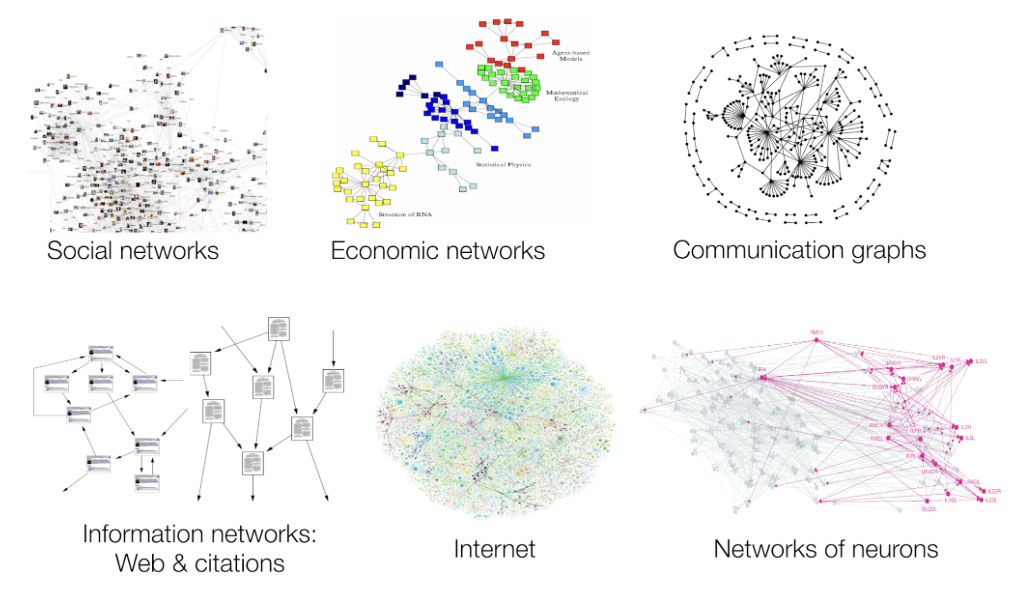
\includegraphics[width=0.7\textwidth]{examples}
    \label{fig:LABEL}
\end{figure}

\section*{Networks as graphs}

\begin{itemize}
	\item \textbf{\textcolor{purple}{Network:}} a real-world system of dependent variables, e.g., 
		\begin{itemize}
			\item WWW is a network of hyperlinked documents
			\item Society is a network of individuals linked by family, friendship, professional ties
			\item Metabolic network is a sum of all chemical reactions in a cell
		\end{itemize}
	\item \textbf{\textcolor{orange}{Graph:}} mathematical abstraction for describing networks
	\item In practice, "network" and "graph" are used interchangeably
	\item You can make a graph out of almost anything (e.g., connect all people whose name starts with the same letter), so must ask: Does this graph correspond to a meaningful network?
\end{itemize}

\newpage

\begin{center}
  {\LARGE \textbf{Types of graphs}}
\end{center}
\vspace{0.5cm}

\section*{Annotations}

\begin{itemize}
	\item Entities: nodes/vertices \textit{V}
	\item Relationships/interactions: edges/links \textit{E}
	\item Entire system: graph \textit{G = (V, E)}
	\item \textcolor{purple}{Node degree, $k_i$:} the number of edges adjacent to node \textbf{\textit{i}}
\end{itemize}

\section*{Types of graphs}

\begin{minipage}{0.45\textwidth}
\textbf{\textcolor{purple}{Undirected}} \\
\textbf{Links:} undirected (symmetrical, reciprocal)
% Quick centered image
\begin{figure}[H]
    \centering
    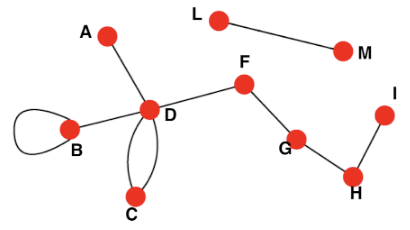
\includegraphics[width=\linewidth]{undirected}
\end{figure}
\textbf{Examples}:
\begin{itemize}
	\item Collaborations
	\item Friendship on Facebook
\end{itemize}
\end{minipage}
\hfill
\begin{minipage}{0.45\textwidth}
\textbf{\textcolor{purple}{Directed}} \\
\textbf{Links:} directed (arcs)
% Quick centered image
\begin{figure}[H]
    \centering
    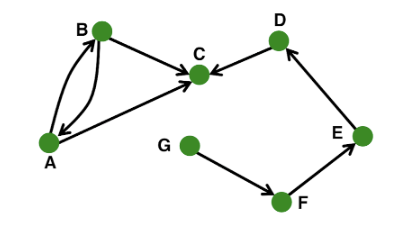
\includegraphics[width=\linewidth]{directed}
\end{figure}
\textbf{Examples:}
\begin{itemize}
	\item Phone calls
	\item Following on Twitter
\end{itemize}
\end{minipage}

\section*{Average node degree}
\begin{minipage}{0.45\textwidth}
\textbf{\textcolor{purple}{Undirected}}
% Quick centered image
\begin{figure}[H]
    \centering
    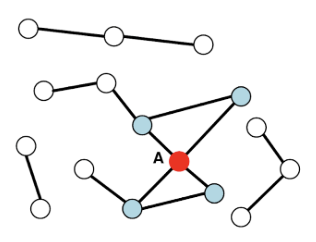
\includegraphics[width=0.6\linewidth]{undirected-example}
\end{figure}

\textbf{\textcolor{purple}{Avg. degree:}} \\
$\overline{k} = <k> = \frac{1}{N} \sum\limits_{i=1}^{N}k_i = \frac{2E}{N}$

\textbf{Intuition}: Every edge increases the sum by 2. Every edge increases the degree of 2 nodes. 
\end{minipage}
\hfill
\begin{minipage}{0.45\textwidth}
\textbf{\textcolor{purple}{Directed}}

In directed networks we define an \textbf{in-degree} and \textbf{out-degree}. The (total) degree of a node is the sum of in- and out-degrees.
% Quick centered image
\begin{figure}[H]
    \centering
    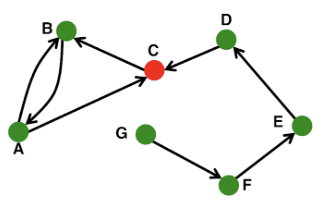
\includegraphics[width=0.6\linewidth]{directed-example}
\end{figure}
$k^{in}_C = 2$ \hspace{0.5cm} $k^{out}_C = 1$ \hspace{0.5cm} $k_C = 3$ \\

\textbf{\textcolor{purple}{Avg. degree:}}  ⏎

$\overline{k} = \frac{E}{N}$ \hspace{0.5cm} $\overline{k^{in}} = \overline{k^{out}}$
\end{minipage}

\begin{minipage}{0.45\textwidth}
\textbf{\textcolor{pink}{Unweighted}} 

(undirected)

% Quick centered image
\begin{figure}[H]
    \centering
    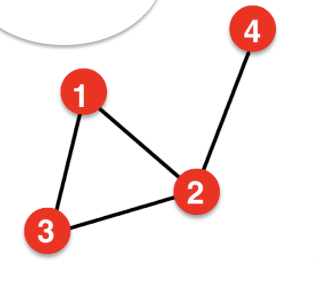
\includegraphics[width=0.5\textwidth]{undirected-unweighted}
    \label{fig:LABEL}
\end{figure}

\textcolor{green}{\textbf{Examples:} Friendship, Hyperlink}
\end{minipage}
\hfill
\begin{minipage}{0.45\textwidth}
\textbf{\textcolor{blue}{Weighted}}

(undirected)

% Quick centered image
\begin{figure}[H]
    \centering
    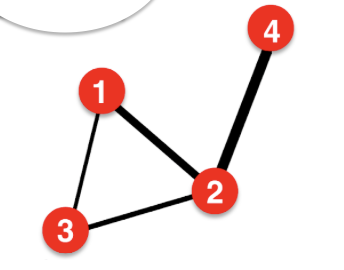
\includegraphics[width=0.5\textwidth]{undirected-weighted}
    \label{fig:LABEL}
\end{figure}

\textcolor{green}{\textbf{Examples:} Collaboration, Internet, Roads}
\end{minipage}

\begin{minipage}{0.6\textwidth}
\begin{itemize}
	\item \textbf{\textcolor{green}{Bipartite graph}} is a graph whose nodes can be divided into two disjoint sets \textbf{\textit{U}} and \textbf{\textit{V}} such that every link connects a node in \textbf{\textit{U}} to one in \textbf{\textit{V}} \\
	\item \textbf{\textcolor{blue}{Examples:}}
		\begin{itemize}
			\item Authors-to-Papers (they authored)
			\item Actors-to-Movies (they appeared in)
			\item Users-to-Movies (they rated)
			\item Recipes-to-Ingredients (they contain) \\
		\end{itemize}
	\item \textbf{\textcolor{pink}{"Folded" networks (a.k.a. "projections"):}}
		\begin{itemize}
			\item Author collaboration networks
			\item Movie co-rating networks
		\end{itemize}
\end{itemize}
\end{minipage}
\hfill
\begin{minipage}{0.3\textwidth}
\centering
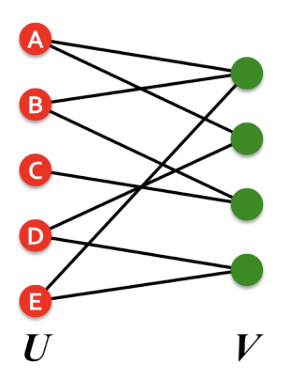
\includegraphics[width=\linewidth]{biparte}
\end{minipage}

\textbf{\textcolor{red}{Projects of bipartite graph}}
% Quick centered image
\begin{figure}[H]
    \centering
    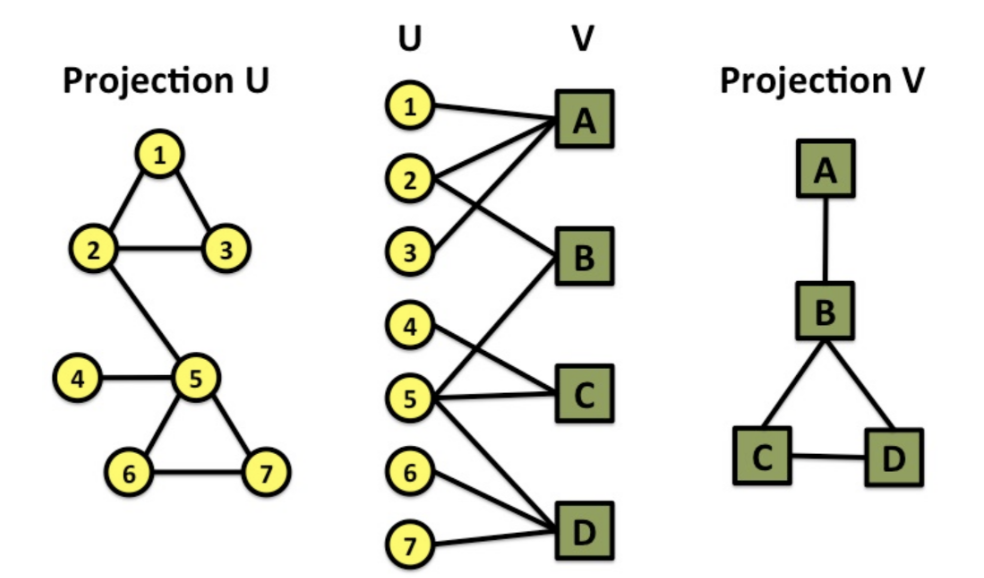
\includegraphics[width=0.7\textwidth]{bipartite-projection}
    \label{fig:LABEL}
\end{figure}

\newpage

\begin{center}
  {\LARGE \textbf{Representing graphs on computers}}
\end{center}
\vspace{0.5cm}

\section*{Adjacency matrix}
\begin{minipage}{0.5\textwidth}
% Quick centered image
\begin{figure}[H]
    \centering
    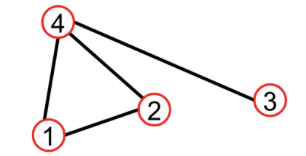
\includegraphics[width=0.6\textwidth]{adjacency-matrix-undirected}
    \label{fig:LABEL}
\end{figure}
\end{minipage}
\hfill
\begin{minipage}{0.5\textwidth}
% Quick centered image
\begin{figure}[H]
    \centering
    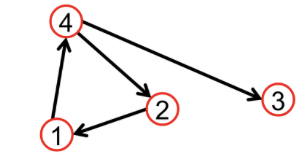
\includegraphics[width=0.6\textwidth]{adjacency-matrix-directed}
    \label{fig:LABEL}
\end{figure}
\end{minipage}

\hspace{1cm} $\mathbf{A_{ij} = 1}$ if there is a link from node \textit{\textbf{i}} to node \textbf{\textit{j}} 

\hspace{1cm} $\mathbf{A_{ij} = 0}$ otherwise

\begin{minipage}{0.5\textwidth}
\[
	A = 
	\begin{pmatrix}
		0 & 1 & 0 & 1 \\
		1 & 0 & 0 & 1 \\
		0 & 0 & 0 & 1 \\
		1 & 1 & 1 & 0 \\
	\end{pmatrix}
.\] 
\end{minipage}
\begin{minipage}{0.5\textwidth}
\[
	A = 
	\begin{pmatrix}
		0 & 0 & 0 & 1 \\
		1 & 0 & 0 & 0 \\
		0 & 0 & 0 & 0 \\
		0 & 1 & 1 & 0 \\
	\end{pmatrix}
.\] 
\end{minipage}

\textcolor{green}{Note that for a directed graph (right) the matrix is not symmetric}

But for big graphs... \textbf{\textcolor{red}{adjacency matrix is usually sparse}}! \textcolor{blue}{What is a better representation?}

\section*{Edge list}
\textbf{Represent a graph as a set of edges}

\begin{minipage}{0.3\textwidth}
\begin{itemize}
	\item (2, 3)
	\item (2, 4)
	\item (3, 2)
	\item (3, 4)
	\item (4, 5)
	\item (5, 2)
	\item (5, 1) \\
\end{itemize}

Here we only need \textit{E} entries to store the same information! 
\end{minipage}
\begin{minipage}{0.3\textwidth}
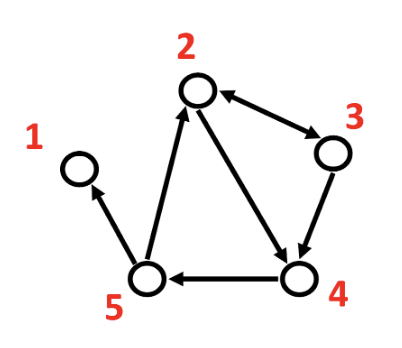
\includegraphics[width=\linewidth]{edge-list}
\end{minipage}

\section*{Adjacency list}

\textbf{\textcolor{blue}{Adjacency list:}}
\begin{itemize}
	\item Easier to work with if network is:
		\begin{itemize}
			\item Large
			\item Sparse
		\end{itemize}
\end{itemize}

\begin{minipage}{0.6\textwidth}
Allows use to quickly retrieve all neighbors of a given node \\

\begin{itemize}
	\item 1:
	\item 2: 3, 4
	\item 3: 2, 4
	\item 4: 5
	\item 5: 1, 2
\end{itemize}

\end{minipage}
\hfill
\begin{minipage}{0.3\textwidth}
\centering
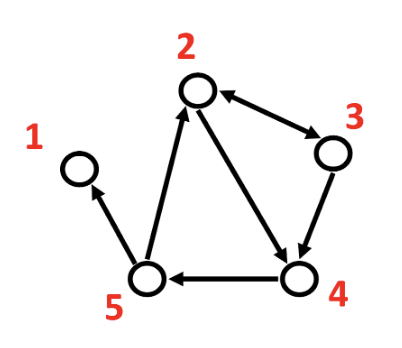
\includegraphics[width=\linewidth]{edge-list}
\end{minipage}

\vspace{0.5cm}

\begin{center}
  {\LARGE \textbf{Properties of real-world networks}}
\end{center}
\vspace{0.5cm}

\begin{itemize}
	\item Real networks are different from arbitrary graphs
	\item Real networks tend to share certain properties
	\item Remarkable, given the diversity of netwokrs
		\begin{itemize}
			\item Information networks (e.g., Web graph, knowledge graphs)
			\item Social networks (e.g., Facebook, dating networks)
			\item Biological networks (e.g., protein-protein interaction)
			\item etc...
		\end{itemize}
\end{itemize}

\section*{sparsity}
\begin{itemize}
	\item Every node connected to only small fraction of all nodes
	\item i.e., $k_i << N$
	\item Often bounded by a constant
		\begin{itemize}
			\item e.g., social networks: Dunbar's number (cognitive limit to the number of people with whom one can maintain stable social relationships; allegedly 150)
		\end{itemize}
\end{itemize}

\section*{degree distribution}

\textbf{\textcolor{purple}{Degree distribution \textit{P(k)}}}: Probability that a randomly chosen node has degree \textbf{\textit{k}}

\hspace{0.3cm} \textit{\textbf{$N_k$}} = $\#$ nodes with degree \textit{\textbf{k}} 

Normalized histogram: 

\hspace{0.3cm} \textbf{\textit{P(k) = $\mathbf{N_k}$ / N}} $\Rightarrow$ \textbf{\textcolor{purple}{plot}}


Hence, the degree distribution just means what percentage of nodes has a certain degree \textit{\textbf{k}}. 

In a real-world network (social network), it looks more like this:
% Quick centered image
\begin{figure}[H]
    \centering
    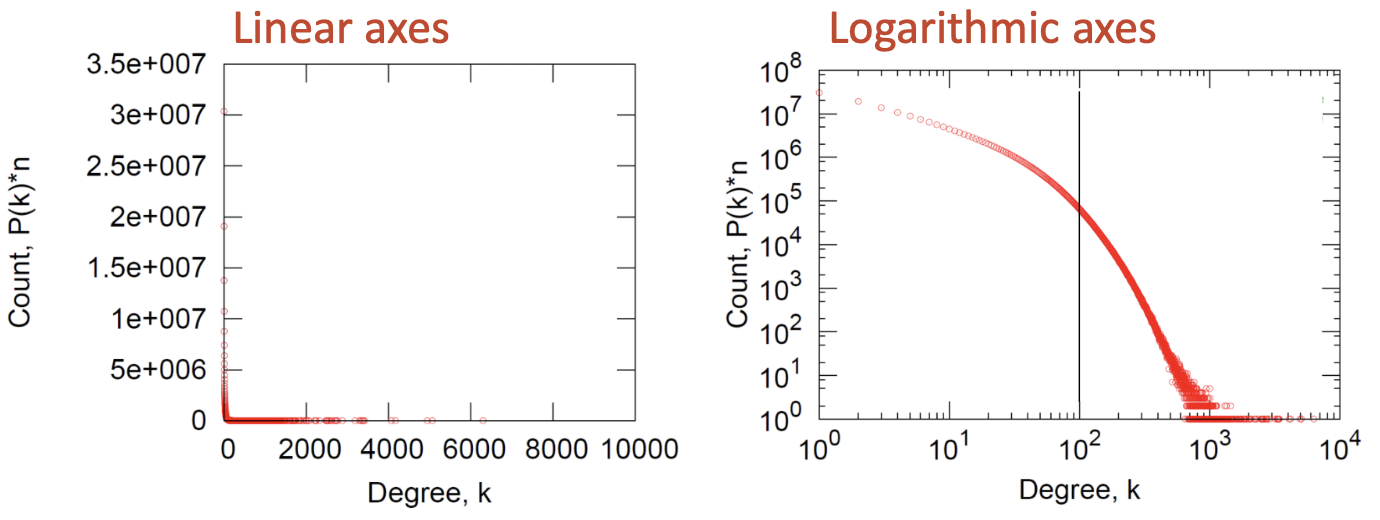
\includegraphics[width=0.8\textwidth]{degree-distribution}
    \label{fig:LABEL}
\end{figure}

\textbf{Common behavior in real-world network}: \underline{power-laws}! 

If we want to quantify to obtain some information, we should use \textbf{median} instead of mean for power laws. Median sometimes is not that informative, so consider using \textbf{average of logarithm, exponentiate and thus obtain the geometric mean.}

\section*{Triadic closure}
\begin{itemize}
	\item "A friend of my friend is my friend"
	\item Measured via clustering coefficient \textit{$C_i$} of node \textit{i}: \\
	$C_i$ =  (\# edges among neighbors of \textit{i}) / (\# potential edges among neighbor of \textit{i})
	\item \# potential edges amount neighbors of \textit{i} in undirected graph: $k_i (k_i - 1) / 2$
\end{itemize}

% Quick centered image
\begin{figure}[H]
    \centering
    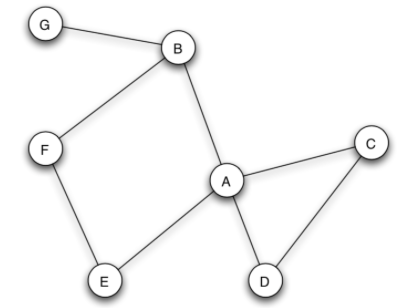
\includegraphics[width=0.25\textwidth]{triadic-closure}
    \label{fig:LABEL}
\end{figure}

\begin{itemize}
	\item $C_A = 1 / (4* 3/2) = 1/6$
	\item In real networks, nodes have \textbf{\textcolor{orange}{large clustering coefficients}}
\end{itemize}

\newpage
\section*{community structure}

\begin{itemize}
	\item Triadic closure makes real networks \textbf{\textcolor{blue}{cluster into locally dense "communities"}}
	\item Communities connected via "weak ties"
	\item Weak ties fill "structural holes"
\end{itemize}

% Quick centered image
\begin{figure}[H]
    \centering
    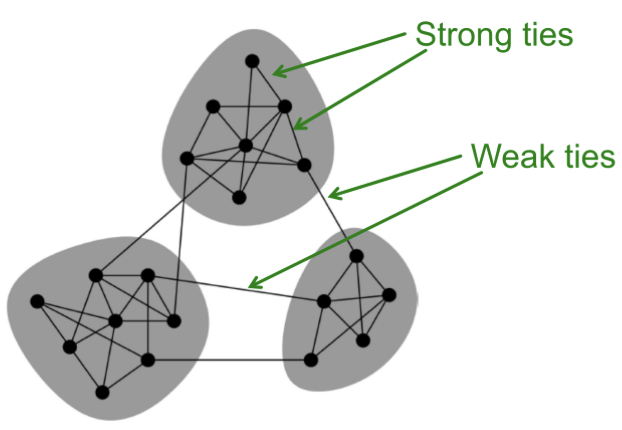
\includegraphics[width=0.5\textwidth]{community-structure}
    \label{fig:LABEL}
\end{figure}

\begin{itemize}
	\item In real life, communities are often not disjoint, but overlapping: 
\end{itemize}
% Quick centered image
\begin{figure}[H]
    \centering
    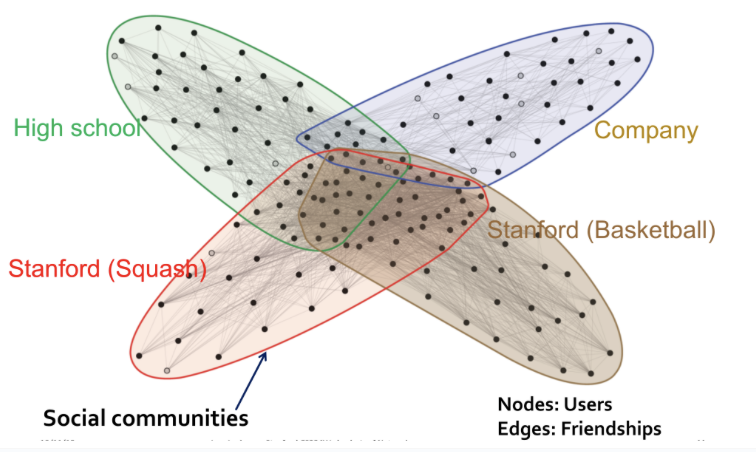
\includegraphics[width=0.6\textwidth]{community-structure-2}
    \label{fig:LABEL}
\end{figure}

\section*{Average shortest-path length}

\begin{itemize}
	\item \textbf{What is the typical shortest path length between any two people?}
		\begin{itemize}
			\item Experiment on the global friendship network
				\begin{itemize}
					\item Can't measure, need to probe explicitly 
				\end{itemize}
		\end{itemize}
	\item \textbf{Small-world experiment}
		\begin{itemize}
			\item Picked 300 people in Omaha, Nebraska
			\item Ask them to get a letter to a stock-broker in Boston by passing it through friends
		\end{itemize}
	\item \textbf{How many steps did it take?}
\end{itemize}

\newpage

% Quick centered image
\begin{figure}[H]
    \centering
    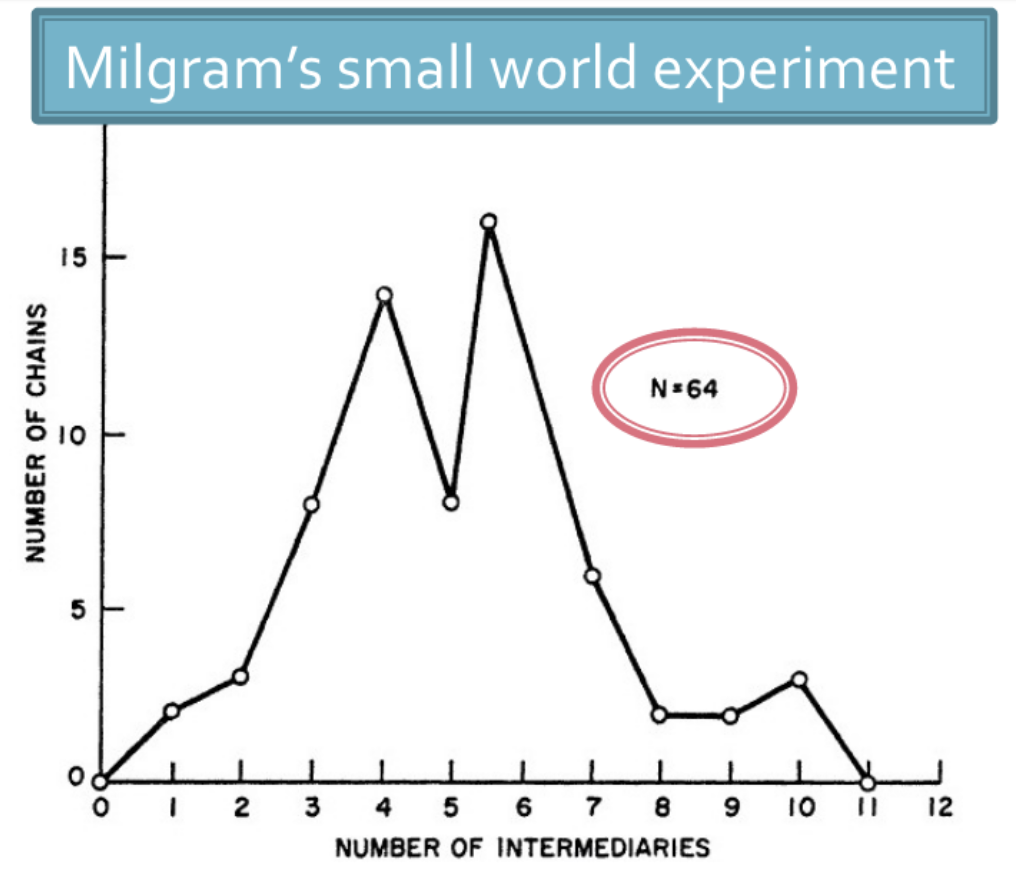
\includegraphics[width=0.5\textwidth]{milgram}
    \label{fig:LABEL}
\end{figure}

\begin{itemize}
	\item \textbf{64 chains completed:} \\
	(i.e., 64 letters reaches the target)
		\begin{itemize}
			\item It took 6.2 steps on the average, thus \textbf{"6 degrees of separation"}.
		\end{itemize}
	\item \textbf{Further observations:}
		\begin{itemize}
			\item People who owned stock had shorter paths to the stockbroker than random people: 5.4 vs 6.7
			\item People from the Boston area have been closer paths: 4.4
		\end{itemize}
\end{itemize}

\section*{Navigability}

\begin{itemize}
	\item For decades, people focused on the fact that short paths exist in social networks
	\item But this is true even in random graphs
	\item The truly amazing fact is not that short paths exist, but that they are discoverable via greedy decentralized routing (as in Milgram's experiment)
	\item Example: \underline{Wikispeedia}: Play a game and see for yourself how well you can navigate an a-priori unknown network.
\end{itemize}

\section*{Homophily/heterophily}

\begin{minipage}{0.6\textwidth}
\begin{itemize}
	\item "Birds of a feather flock together"
	\item Especially in social networks
	\item Big confound and cause of debate: Influence vs. homophily
	\item E.g., obese people's friends are more likely to also be obese
		\begin{itemize}
			\item Influence: I copy eating behavior of those around me
			\item Homophily: people with similar eating behavior prone to become friends
		\end{itemize}
\end{itemize}
\end{minipage}
\hfill
\begin{minipage}{0.4\textwidth}
\centering
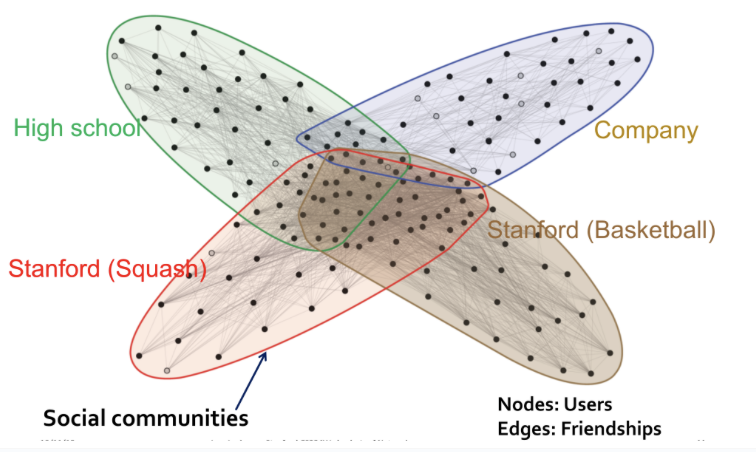
\includegraphics[width=\linewidth]{community-structure-2}
\end{minipage}

\section*{Property of real-world networks: summary}
Real-world networks (across many types)
\begin{itemize}
	\item are sparsely connected,
	\item but some nodes are much more connected than most others (i.e., skewed degree distribution);
	\item form locally dense clusters via triadic closure,
	\item which leads to community structure;
	\item have short paths between random node pairs (partly due to "hubs" [skewed degree distributing!]),
	\item and the short paths are easily discoverable.
\end{itemize}

\vspace{0.5cm}

\begin{center}
  {\LARGE \textbf{Measure node importance}}
\end{center}
\vspace{0.5cm}
\textbf{\textcolor{red}{How to measure "importance" of a node?}}
\begin{itemize}
	\item Formalized via \textit{centrality measures}
	\item Map each node \textit{i} to a scalar value \textit{C(i)} capturing its importance in the overall network
\end{itemize}

\section*{Degree centrality}
\begin{itemize}
	\item Simplest centrality measure
	\item Many neighbors $\Rightarrow$ important node
		\begin{itemize}
			\item \textit{C(i)} = number of neighbors of \textit{i}
		\end{itemize}
	\item Very brittle, easy to "rig"
		\begin{itemize}
			\item E.g., Twitter: scam account, followed by 100,000 other scam accouns
		\end{itemize}
\end{itemize}

\section*{Closeness centrality}
\begin{itemize}
	\item Farness(x) = total distance to x from other nodes
	\item C(x) = 1 / Farness(x) \\
		\[
			C(x) = \frac{1}{\sum_y d(y, x)}
		.\] 
		\begin{itemize}
			\item Reciprocal to turn farness into closeness
			\item Only defined for connected graphs (otherwise \textit{d} infinite)
		\end{itemize}
	\item Under \textcolor{orange}{closeness centrality}, nodes that are easy to reach from anywhere in the network are considerer important
	\item Variant: \textcolor{purple}{harmonic centrality}: switch sum and reciprocal \\
		\[
			C(x) = \sum\limits_{y \neq x} \frac{1}{d(y, x)}
		.\] 
		\begin{itemize}
			\item C(x) = total reciprocal distance to x to other nodes
			\item Defined even for disconnected graphs \\
			(define \textit{1/d} of disconnected nodes as 0)
		\end{itemize}	
\end{itemize}

\section*{Betweenness centrality}
\begin{itemize}
	\item \textit{C(i)} = average fraction of all shortest paths in the network that pass through node \textit{i}
	\item Computation of betweenness centrality of node \textit{i}:
		\begin{itemize}
			\item For each pair of vertices \textit{(s, t)}: 
				\begin{itemize}
					\item Find all shortest paths from \textit{s} to \textit{t}
					\item Compute the fraction of these shortest paths that pass through \textit{i}
				\end{itemize}
			\item Average this fraction over all pairs of vertices\textit{(s, t)}
		\end{itemize}
	\item Expensive to compute
\end{itemize}

\section*{Katz centrality}
\begin{itemize}
	\item Generalization of degree centrality
	\item Degree centrality counts only number of direct neighbors (i.e., neighbors at distance 1)
	\item Katz centrality also counts neighbors at distances 2, 3, ...
	\item More precisely, number of paths from other nodes to \textit{i}, giving less weight to larger distances: \\
		\[
			C(i) = \sum\limits_{k=1}^{\infty} \sum\limits_{j=1}^{N} \alpha^{k} (A^{k})_{ji}
		.\] 
	\begin{tcolorbox}[
	  colback=gray!15,     % background color
	  colframe=black!50,    % border color
	  boxrule=1pt,       % border thickness
	  arc=3mm,             % rounded corners
	  left=4mm, right=4mm, top=2mm, bottom=2mm % padding
	]
	\textit{k}-th power of adjacency matrix \textit{A} contains number of length-\textit{k} paths for each node pair
	\end{tcolorbox}
	\item More robust than degree centrality
\end{itemize}
\section*{PageRank centrality}

\begin{itemize}
	\item Recursive definition: my centrality $C(i) := x_i$ is high if I receive inlinks from many other central nodes:
		\[
			x_i = \sum\limits_j a_{ji} \frac{x_j}{L(j)} 
                \]
		\[
			L(j) = \sum\limits_i a_{ji}
		\] 
		\begin{tcolorbox}[
		  colback=gray!15,     % background color
		  colframe=black!50,    % border color
		  boxrule=1pt,       % border thickness
		  arc=3mm,             % rounded corners
		  left=4mm, right=4mm, top=2mm, bottom=2mm % padding
		]
		$a_{ji}$ : entry \textit{(j, i)} of adjacency matrix \textit{A} (1 if \textit{j} links to \textit{i}, else 0) \\
		\textit{L(j)}: out-degree of \textit{j}
		\end{tcolorbox}
	\item Some extra tweaks to make it work with any graph (e.g., disconnected)
	\item Matrix notation: $\mathbf{x = Mx}$ \\
	(where \textit{M} is computed from adjacency matrix \textit{A})
	\item Do you recognize this?
		\begin{itemize}
			\item \textit{x} is eigenvector of \textit{M} with eigenvalue 1 $\Rightarrow$ we're in linear-algebra land
			\item \textit{x} is the steady state the Markov chain induced by the network: $x_i$ is fraction of time a random walker will have spent in node \textit{i}, after a very long ($\Rightarrow \infty$ random walk
		\end{itemize}
	\item The technology that made Google huge
		\begin{itemize}
			\item "Page" in PageRank for Larry PAge
			\item MapReduce was invented to compute PageRank on full Google Web crawl
		\end{itemize}
	\item Bottom line: Pay attention in your linear algebra class
\end{itemize}


\end{document}
